\section{Cell Envelope Biogenesis}
In contrast to nutrient transporters, which support the synthesis of
biomolecules throughout the cell and therefore need to scale with the cell
size, here we must consider the synthesis of components that will need to
scale with the surface area of the cell. \textit{E. coli} is a rod-shaped
bacterium with a remarkably robust length-to-width aspect ratio of $\approx$
4:1 \citep{harris2018, ojkic2019}. Assuming this surface area is
approximately the same between the inner and outer membranes of \textit{E.
coli}, and the fact that each membrane is itself is a lipid bilayer (or, a
bilayer with lipopolysaccharides decorating the outer membrane), our rule-of-thumb
of 5 \textmu m$^2$ per surface suggests a total membrane surface area of
$\approx 20  $\textmu m$^2$ (see the Appendix Section "Estimation of Cell Size and Surface Area" for a description of the calculation of cell
surface area as a function of cell size). In this section, we will estimate
the number of key protein complexes needed to synthesize the lipids as well
as the complexes involved in assembling the peptidoglycan scaffold that make
up the cell envelope.

\subsection{Lipid Synthesis}
The dense packing of the membrane with proteins means that the cell membranes
are not composed entirely of lipid molecules, with only $\approx$ 40 \% of the
membrane area occupied by lipids or lipopolysaccharide, both of which have fatty
acid chains of similar length (BNID: 100078). Using a rule-of-thumb of 0.5
nm$^2$ as the surface area of the typical lipid (BNID: 106993), we can
estimate $\sim$ 2 $\times$ 10$^7$ lipids per cell, which is in close
agreement with experimental measurements (BNID: 100071, 102996).

The membranes of \textit{E. coli} are composed of a variety of different lipids,
each of which are unique in their structures and biosynthetic pathways
\citep{sohlenkamp2016}. Recently, a combination of stochastic kinetic modeling
\citep{ruppe2018} and \textit{in vitro} kinetic measurements
\citep{ranganathan2012, yu2011} has revealed remarkably slow steps in the fatty
acid synthesis pathways which may serve as the rate limiting reactions for
making new membrane fatty acids (that become components of a variety of
membrane lipids) in \textit{E. coli}. One such step is the removal of hydroxyl
groups from the fatty-acid chain by ACP dehydratase that leads to the formation
of carbon-carbon double bonds. This reaction, catalyzed by proteins FabZ and
FabA \citep{yu2011}, has been estimated to have kinetic
turnover rates of $\approx$ 1 dehydration per second per enzyme
\citep{ruppe2018}. Thus, given this rate and the need to synthesize $\approx$ 2
$\times$ 10$^7$ lipids over 5000 seconds, one can estimate that a typical cell
requires $\approx$ 4000 ACP dehydratases. This is in reasonable agreement with
the experimentally observed copy numbers of FabZ and FabA
(\FIG{cell_envelope}(A)). Furthermore, we can extend this estimate to account
for the change in membrane surface area as a function of the growth rate (grey
line in \FIG{cell_envelope}(A)), which in contrast to our observations with glucose uptake, indeed captures the observed growth rate
dependent expression of these two enzymes.

\subsection{Peptidoglycan Synthesis}
The exquisite control of bacteria over their cell shape is due primarily to a stiff, several nanometer thick meshwork of
polymerized disaccharides that makes up the cell wall termed the peptidoglycan. The formation of the peptidoglycan is an intricate
process involving many macromolecular players \citep{shi2018, morgenstein2015},
whose coordinated action synthesizes the individual subunits and integrates them
into the peptidoglycan network that maintains cell shape and integrity even in the face of
large-scale chemical and osmotic perturbations \citep{harris2018,shi2018}.
Due to the extensive degree of chemical crosslinks between glycan strands, the
entire peptidoglycan is a single molecule comprising $\approx$ 3\% of the cellular dry mass (BNID:
1019360), making it the most massive molecule in \textit{E. coli}. The
polymerized unit of the peptidoglycan is a N-acetylglucosamine and
N-acetylmuramic acid disaccharide, of which the former is functionalized with a
short pentapeptide. With a mass of $\approx$ 1000 Da, this unit, which we refer
to as a murein subunit, is polymerized to form long strands in the periplasm
which are then attached to each other via their peptide linkers. Together, these
quantities provide an estimate of $\approx$ 5 $\times$ 10$^6$ murein subunits
per cell.

There are various steps which one could consider \textit{a priori} to be a
limiting process in the synthesis of peptidoglycan, including the
biosynthesis steps that occur in the cytoplasm, the transglycosylation
reaction which adds new subunits to the glycan strands, and the formation
of the peptide crosslinks between strands
\citep{shi2018,morgenstein2015,lovering2012,barreteau2008}. Despite the
extensive mechanistic characterization of these components,
\textit{quantitative} characterization of the individual reaction rates along
the entire kinetic pathway of remain scarce and make identification of any
particularly slow steps difficult. However, such measurements have recently
been made for the crosslinking machinery [transpeptidases,
\cite{catherwood2020}] of the peptidodglycan which provides lateral
structural integrity to the peptidoglycan shell. As the primary mechanism of
subunit integration occurs by a complex with both transglycosylation and
transpeptidation activities \citep{shi2018} and that the measured turnover of
transpeptidases being rather slow ($\approx$ 2 crosslinking reactions per
second) we therefore consider only the transpeptidation reaction in this
work. We believe that, in lieu of other quantitative measurements,
crosslinking represents a reasonable candidate for a rate-limiting step in
growth as it is vital for cell size and shape homeostasis.

In principle, each murein subunit can be involved in such a crosslink. In
some microbes, such as in Gram-positive bacterium \textit{Staphylococcus
aureus}, the extent of crosslinking can be large with $>$ 90\% of
pentapeptides forming a connection between glycan strands. In \textit{E.
coli}, however, a much smaller proportion ($\approx$ 20\%) of the peptides
are crosslinked, resulting in a weaker and more porous cell wall
\citep{vollmer2008a, rogers1980}. The formation of these crosslinks occurs
primarily during the polymerization of the murein subunits and is facilitated
by a family of transpeptidase enzymes. The four primary transpeptidases of
\textit{E. coli} have only recently been quantitatively characterized
\textit{in vivo}, via liquid chromatography mass spectrometry, which revealed
a notably slow kinetic turnover rate of $\approx 2$ crosslinking reactions
formed per second per enzyme as  noted above \citep{catherwood2020}.

Assembling these quantities permits us to make an estimate that on the order
of $\approx$ 100 transpeptidases per cell are needed for complete maturation
of the peptidoglycan, given a division time of $\approx$ 5000 seconds; a
value that is comparable to experimental observations
[\FIG{cell_envelope}(B)]. Expanding this estimate to account for the changing
mass of the peptidoglycan as a function of growth rate [grey line in
\FIG{cell_envelope}(B)] predicts an order-of-magnitude increase in the
abundance of the transpeptidases when the grow rate is increased by a factor
of four. Here, however, the measured complex abundances across the different proteomic data sets show systematic disagreements and obfuscates any significant dependence on growth rate.

\subsubsection{Limits on Cell Wall Biogenesis}
While the processes we have considered represent only a small portion of
proteins devoted to cell envelope biogenesis, we find it unlikely that they
limit cellular growth in general. The relative amount of mass required for
lipid and peptidoglycan components will decrease at faster growth rates due to a
decrease in the cell's surface area to volume (S/V) ratio \citep{ojkic2019}.
Furthermore, despite the slow catalytic rate of FabZ and FabA in lipid
synthesis, experimental data and recent computational modeling has shown that
the rate of fatty-acid synthesis can be drastically increased by increasing
the concentration of FabZ \citep{yu2011, ruppe2018}. With a proteome size of
$\approx$ 3$\times$10$^6$ proteins, a hypothetical 10-fold increase in
expression from 4000 to 40,000 ACP dehydratases would result in a paltry
$\approx$ 1\% increase in the size of the proteome. In the context of
peptidoglycan synthesis, we note that our estimate considers only the
transpeptidase enzymes that are involved in lateral and longitudinal elongation
of the peptidoglycan. This neglects the presence of other transpeptidases
that are present in the periplasm and also involved in remodeling and
maturation of the peptidoglycan. It is therefore possible that if this was
setting the speed limit for cell division, the simple expression of more
transpeptidases would be sufficient to maintain the structural integrity of the
cell wall.

\begin{figure}
    \begin{fullwidth}
    \centering{
    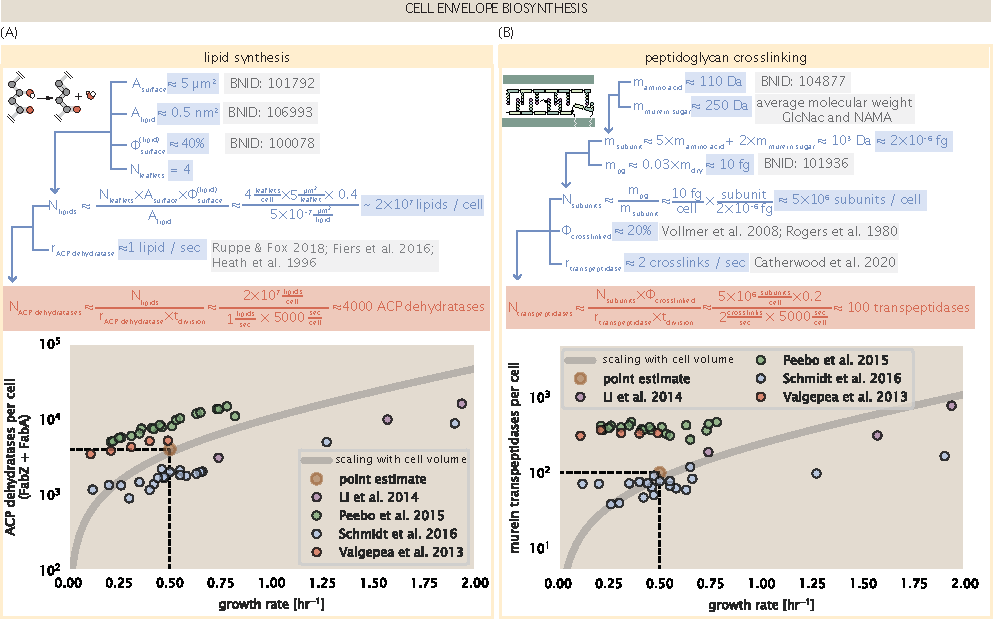
\includegraphics{main_figs/fig3_cell_wall_peptidoglycan.pdf}
    \caption{(A) Top panel shows an estimation for the
            number of ACP dehydratases necessary to form functional
            phospholipids, which is assumed to be a rate-limiting step on
            lipid synthesis. The rate of ACP dehydratases was inferred from
            experimental measurements via a stochastic kinetic model
            described in \cite{ruppe2018}. Bottom panel shows the
            experimentally observed complex copy numbers using the
            stoichiometries [FabA]$_2$ and [FabZ]$_2$. (B) An estimate for
            the number of peptidoglycan transpeptidases needed to complete
            maturation of the peptidoglycan. The mass of the murein subunit
            was estimated by approximating each amino acid in the
            pentapeptide chain as having a mass of 110 Da and each sugar in
            the disaccharide having a mass of $\approx$ 250 Da. The
            \textit{in vivo} rate of transpeptidation in \textit{E. coli}
            was taken from recent analysis by \cite{catherwood2020}. The
            bottom panel shows experimental measurements of the
            transpeptidase complexes in \textit{E. coli} following the
            stoichiometries [MrcA]$_2$, [MrcB]$_2$, [MrdA]$_1$, and
            [MrdB]$_1$. Grey curves in each plot show the estimated number of
            complexes needed to satisfy the synthesis requirements scaled by
            the surface area as a function of growth
            rate.}
            \label{fig:cell_envelope}
    }
    \end{fullwidth}
\end{figure}
